%!TEX root = ../../thesis.tex
\chapter{SYSTEM DESIGN}

\section{ Architectural Diagram }
In this chapter of the thesis, the proposed system design will be presented and discussed. The architecture of the proposed system design is illustrated in \ref{fig:sys_arch}

\begin{figure}
    \centering
    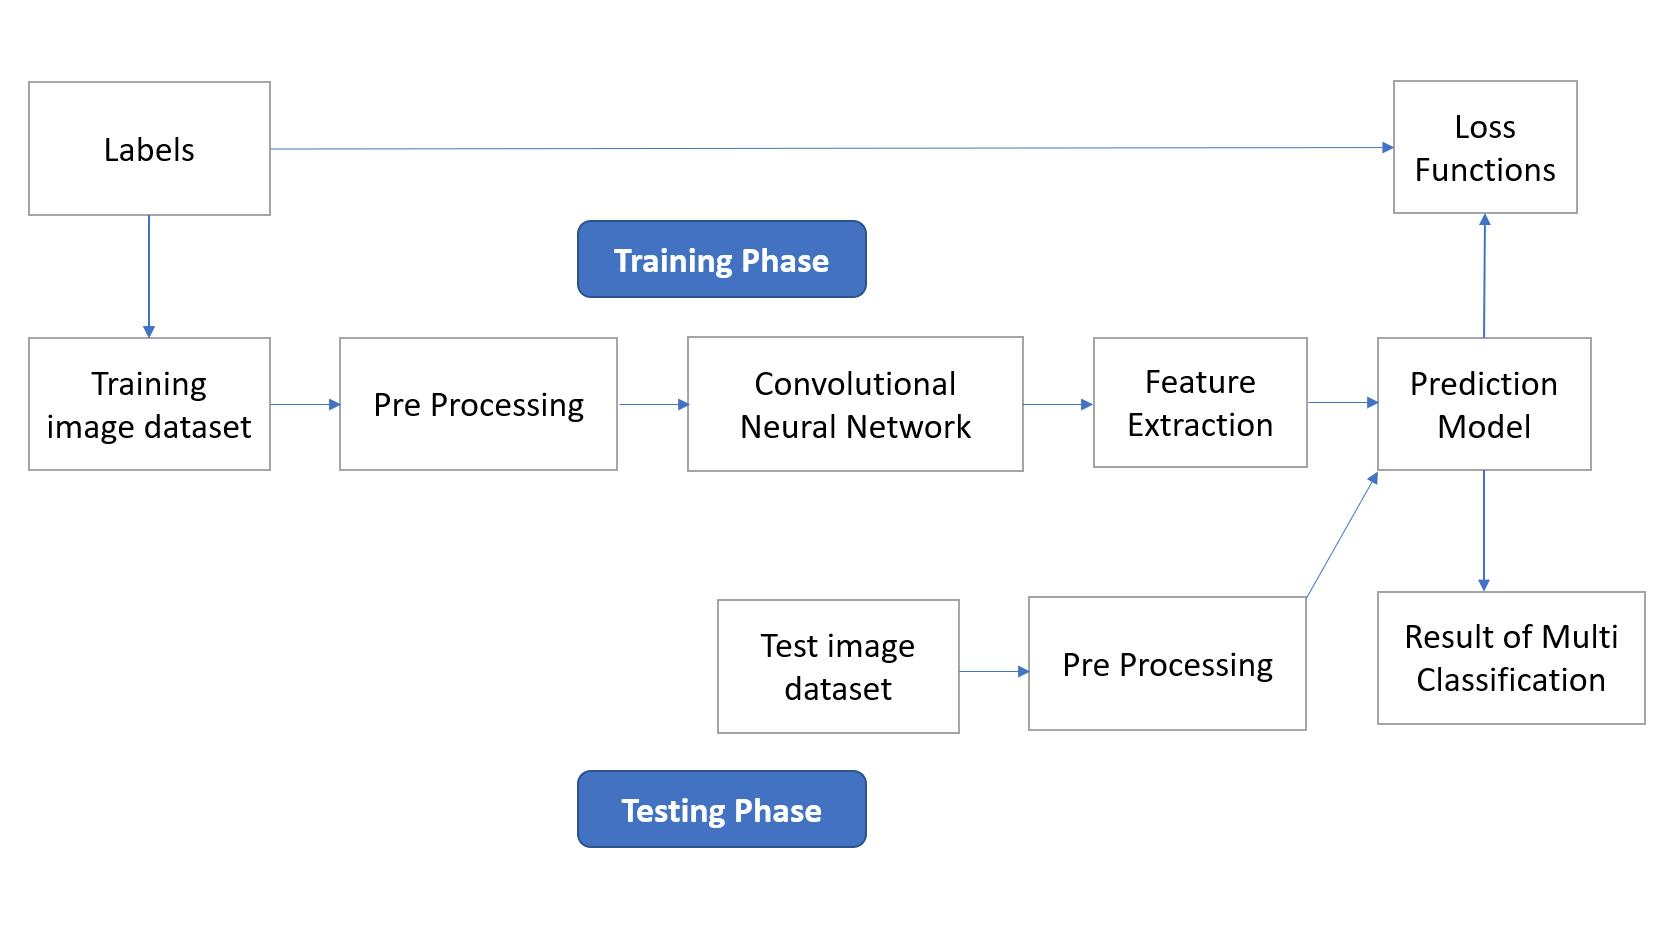
\includegraphics[width=0.60\textwidth]{Img/Chap-01/9.jpg}
    \caption{The System Architecture}
    \label{fig:sys_arch}
\end{figure}

\section{Processing Steps}

The first step is pre-processing which is the stage that converts the picture according to the requirements of the following level. It cleans up the picture by removing noise and other blemishes and sharpening the image's edges. RGB to grey conversion and reshaping are carried out through this stage also, it has a noise-removal feature that uses a median filter. Modern MRI scans have very low noise arrival probabilities. It may show up as a result of the heat effect. In this study, the primary focus is on identifying and classifying tumor cells. Noise reduction is required for the full system, though.


\section{K-Means Clustering for Segmentation}
The steps for k-means clustering are illustrated below:
\begin{enumerate}[a)]
    \item $K$ is the number of clusters.
    \item Pick the $k$ cluster centers at random.
    \item Calculate the cluster's average or center.
    \item Determine the separation between the center of each cluster and each pixel.
    \item If the distance is near the center, go to the closest cluster to the center.
    \item Move on to the next cluster if you can't find what you need.
    \item Calculate the center of gravity again.
    \item Repeat the operation till the center doesn't shift.
\end{enumerate}

\section{Approximate Reasoning}

To estimate the tumor size, the linearization approach is used in the first stage of deductive reasoning. In other words, it's a picture with just two possible colors: black or white (0 or 1). After this, define the tumor's stage and forecast its prognosis from the supplied tumor area.

\section{UML Diagrams}
\subsection{Use Case Diagram}

The use case diagram, as shown in\ref{fig:use_case_example}, can be used to summarize the data about your system's users (also referred to as actors) and their interaction with it. A useful use case diagram can help your team represent and discuss \ref{fig:use_case_example}:
\begin{enumerate}[a)]
    \item Representing the objectives of user-system interactions
    \item Defining and structuring a system's functional needs
    \item Defining a system's context and needs
    \item Modeling the basic flow of events in a use case
\end{enumerate}

\begin{figure}
    \centering
    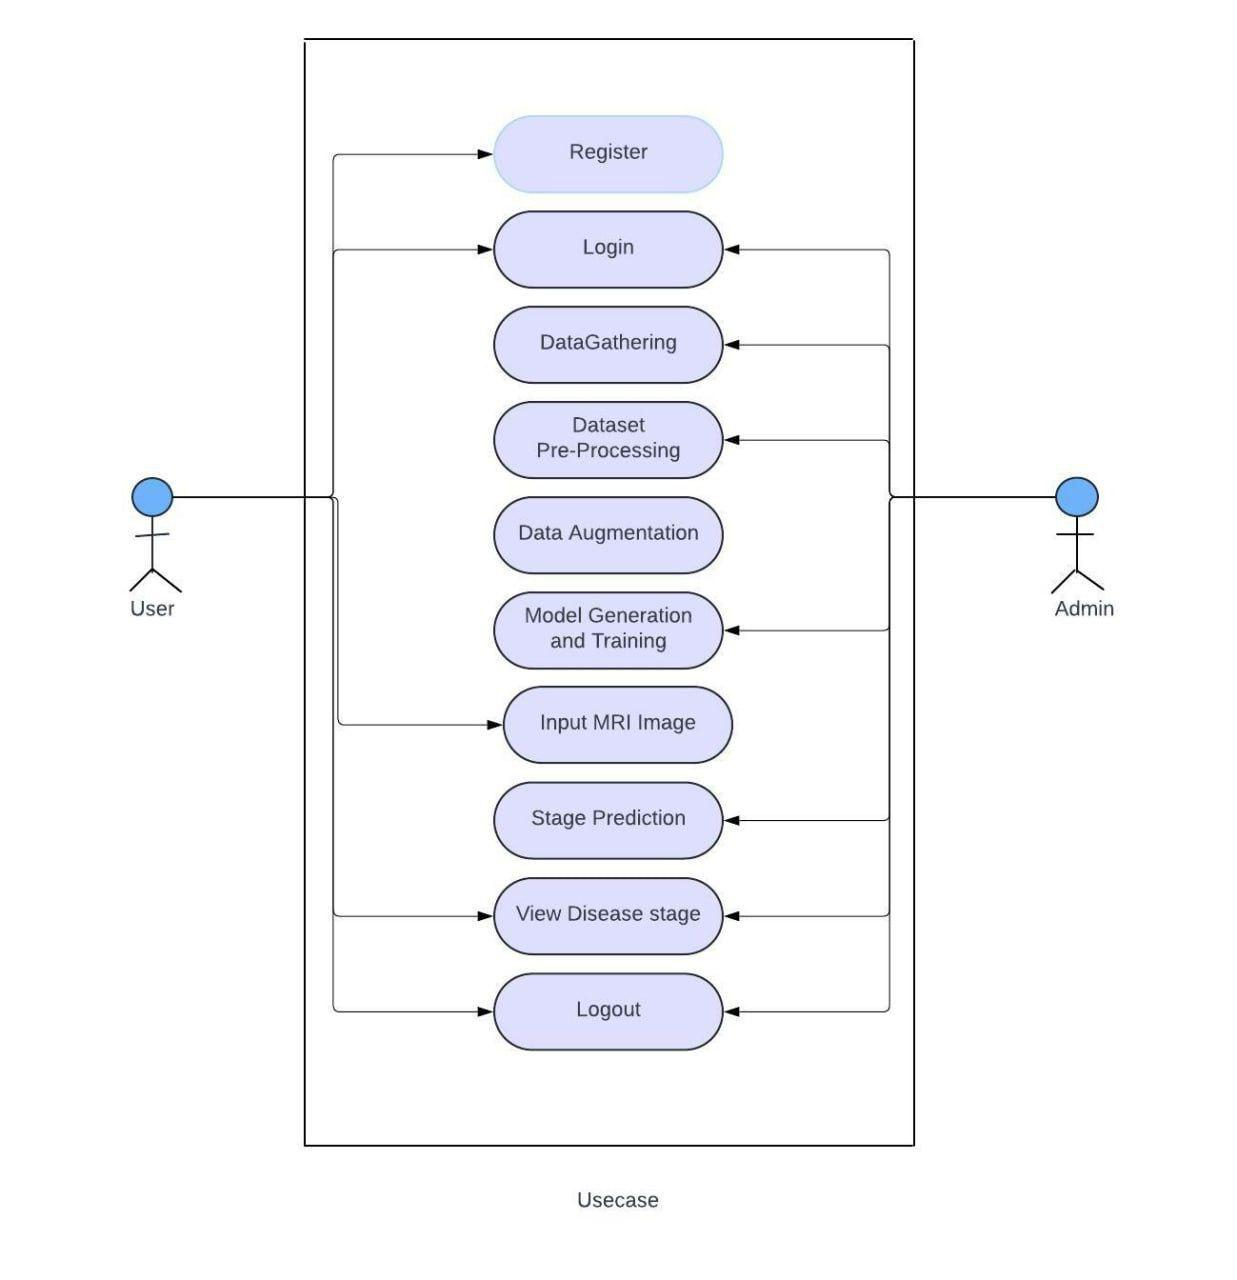
\includegraphics[width=0.60\textwidth]{Img/Chap-01/10.jpg}
    \caption{Use case diagram \cite{mohapatra-54}}
    \label{fig:use_case_example}
\end{figure}

The connection between a system and a user is graphically depicted in a use case diagram. So many user types and their interactions with a system could be depicted in a use case diagram. Internal and external factors are taken into account while drawing up use case diagrams. The majority of these criteria are design specifications. Usage cases are produced, and actors are identified when a system's capability is examined to prepare them for use. The following are some possible uses for use case diagrams:

\begin{enumerate}[i)]
    \item Gathers system requirements.
    \item To acquire a different perspective on a system.
    \item Identify the external and internal elements that affect the system.
    \item Display the performers' interplay.
\end{enumerate}

\section{Sequence Diagram}

A sequence diagram is an interaction diagram that shows how and in what order the processes interact. This is the construction of message sequence diagrams, sometimes called event diagrams, event scenarios, and sequence diagrams.

\section{Activity Diagram}

An activity diagram is a graphical representation of workflows of stepwise activities and actions with support for choice, iteration, and concurrency. An activity diagram shows the overall flow of control \ref{fig:activity_example}. 

The most important shape types: 
\begin{itemize}
    \item Rounded rectangles represent activities.
    \item Diamonds represent decisions. 
    \item Bars represent the start or end of concurrent activities. 
    \item A black circle represents the start of the workflow. 
    \item An encircled circle represents the end of the workflow. 
\end{itemize}


\begin{figure}
    \centering
    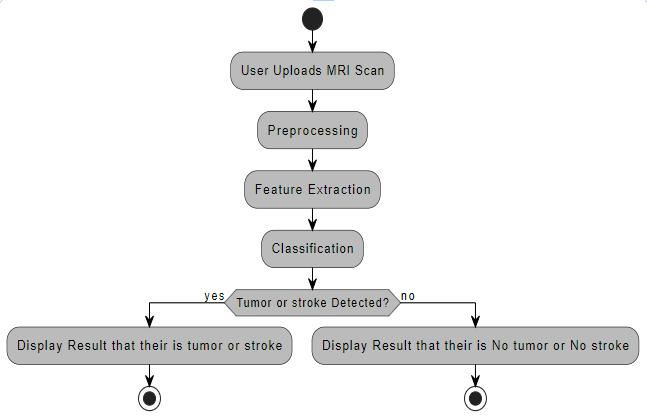
\includegraphics[width=0.60\textwidth]{Img/Chap-01/12.jpg}
    \caption{Activity Diagram}
    \label{fig:activity_example}
\end{figure}

The order of events is shown by arrows that go from the beginning to the finish. As a result, they might be seen as a type of flowchart. It is difficult to express concurrency in flowcharts because of the absence of structures. This can only be resolved for basic 
circumstances by using the join and split symbols in activity diagrams; the model's meaning is obscured when they are arbitrarily coupled with choices or loops. 
Here we upload the image, whether it is of a brain tumor or stroke. It goes through the process of pre-processing, feature extraction, and then classification. Here, in the case of a brain tumor or stroke, the result appears as the presence of the disease, and in the case of the absence of the disease, the result appears as the absence of the disease.

\section{Class Diagram}

Static diagrams, such as the class diagram, are used in textbooks. It's a representation of the application's "static" state. It is possible to create executable code from a class diagram in addition to visualizing, explaining, and documenting many parts of a system. The class diagram is a graphic depiction of a class's attributes, capabilities, and constraints. Class diagrams are frequently used in the design of object-oriented systems as they are the only UML diagrams that may be immediately converted to object-oriented languages. In-class diagrams, relationships, classes, and interfaces may all be viewed. Also displayed are restrictions. Another term for it is a structure diagram. The class diagram serves as a visual representation of an application's static view. \ref{fig:class_diagram_example} shows a diagram showing how processes interact with each other and in what order they do so. As the name suggests, it's based on a Message Sequence Chart construct. The interactions between items are displayed chronologically in a sequence diagram. We can identify the objects and classes that are involved as well as the order of messages that need to be passed between them in this diagram to achieve the objectives of the scenario. Logical View use case realizations are generally depicted in sequence diagrams. Events and scenarios are sometimes used 
interchangeably with sequence diagrams. 

\begin{figure}
    \centering
    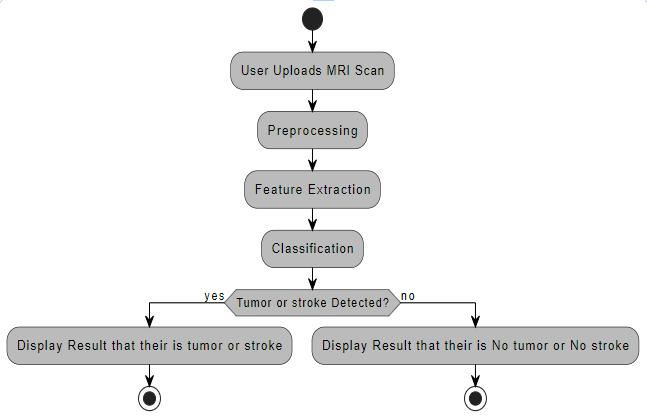
\includegraphics[width=0.60\textwidth]{Img/Chap-01/12.jpg}
    \caption{Class Diagram}
    \label{fig:class_diagram_example}
\end{figure}